% PCA-Matryoshka for vector-database compression -- PVLDB submission.
% PVLDB uses the ACM acmart class (sigconf). Compile with pdflatex.
% Keeps the IEEE/TechRxiv version (pca_matryoshka_ieee_tai.tex) intact.
\documentclass[sigconf, nonacm]{acmart}
\settopmatter{printacmref=false}
\setcopyright{none}
\renewcommand\footnotetextcopyrightpermission[1]{}
\pagestyle{plain}

\usepackage{booktabs}
\usepackage{balance}

\begin{document}

\title{Training-Free Vector-Database Compression: PCA-Matryoshka Truncation and
Scalar Quantization at OPQ-Class Recall and a Fraction of the Build Cost}

\author{Andrew H. Bond}
\affiliation{%
  \institution{San Jose State University}
  \city{San Jose}\state{CA}\country{USA}}
\email{andrew.bond@sjsu.edu}

\begin{abstract}
Billion-scale vector databases pay for every byte: the embedding store dominates
RAM and storage cost, yet most deployed embedding models cannot be truncated --
na\"ive dimension reduction destroys retrieval quality, because only models
trained with a Matryoshka objective place useful information in their leading
dimensions. We present \textbf{PCA-Matryoshka}, a \emph{training-free} technique
that applies a PCA rotation to an embedding model's output so that truncation
becomes effective without retraining (na\"ive truncation of BGE-M3 to 256-d:
cosine $0.467$; with PCA-Matryoshka: $0.974$). Combined with scalar quantization,
it compresses embeddings $\sim$30$\times$ for vector search. On real corpora --
199k LaBSE embeddings and \textbf{1M multilingual Project Gutenberg passages} --
PCA-Matryoshka matches OPQ and \emph{exceeds} the 2024 binary-quantization SOTA,
RaBitQ, on recall@10 ($0.999$ vs $0.962$ with rerank), both far above plain PQ
and IVF-PQ, while
\textbf{building the index 4--20$\times$ faster} because it needs a single
eigen-decomposition rather than OPQ's iterative rotation-plus-codebook
optimization. A batched AVX2 asymmetric-distance kernel searches the compressed
codes at \textbf{3683 qps} (recall@10 $0.9995$, 96\,B/vector) -- $7.9\times$ over
naive decompress-and-scan -- so the method is fast, compressed, and high-recall at
once. We also report a methodological finding with implications for how
the community evaluates compression: \emph{cosine similarity to the original
vector is not a reliable proxy for retrieval quality} at high compression. The
method ships as an open-source system with native PostgreSQL/\texttt{pgvector}
search over compressed vectors, and a one-click reproduction notebook.
\end{abstract}

\keywords{vector databases, approximate nearest neighbor search, embedding
compression, dimension reduction, information retrieval}

\maketitle

\section{Introduction}
Embedding-based retrieval underpins modern search, recommendation, and
retrieval-augmented generation. At scale the cost is dominated not by query
compute but by the \emph{vector store}: hundreds of gigabytes of float32
embeddings in RAM or on SSD. Compression is therefore a first-class
data-management problem.

A tempting lever is \emph{truncation}: keep the first $d'$ of $d$ dimensions.
This works only for models trained with a Matryoshka objective~\cite{mrl}, which
deliberately front-loads information; the overwhelming majority of deployed
encoders (BGE-M3, E5, older OpenAI models) were not, and na\"ive truncation
destroys recall.

\textbf{Contributions.} (1) \textbf{PCA-Matryoshka}, a training-free PCA rotation
that restores the truncation property for \emph{any} encoder, combined with
scalar quantization for $\sim$30$\times$ compression. (2) A fair, two-stage
evaluation on real corpora up to \textbf{1M multilingual vectors} showing
PCA-Matryoshka \emph{ties OPQ and beats the 2024 SOTA RaBitQ on recall while
building 4--20$\times$ faster}, and beating PQ and IVF-PQ. (3) A methodological
result: cosine-to-original is not a reliable proxy for retrieval quality under
aggressive compression. (4) An open-source system with native
\texttt{pgvector} search over compressed vectors and a reproduction notebook.

\section{Method}
PCA-Matryoshka fits a PCA on a sample of the corpus and rotates every embedding
into the principal-component basis, ordering dimensions by explained variance so
that a prefix of length $d'$ retains the dominant signal. The rotated, truncated
vector is then scalar-quantized to $b$ bits with a per-corpus codebook and
bit-packed; the L2 norm is preserved alongside the packed bits. The compact codes
form the RAM-resident index; we report \emph{single-stage} recall (ranking the
codes directly) as the pure-compression operating point. An optional second stage
reranks a small candidate set against the full vectors -- kept on cheaper
storage, as in disk-based ANN -- trading one disk fetch for higher recall. The
pipeline is \emph{training-free}: a single eigen-decomposition, no gradient
training and no iterative codebook optimization.

\section{Experiments}
\textbf{Setup.} Real corpora: (i) 199{,}000 LaBSE embeddings (768-d); (ii)
\textbf{999{,}000 LaBSE embeddings} of passages drawn from Project Gutenberg
(multilingual). 1{,}000 held-out queries, exact cosine ground truth. We compare
against faiss PQ, OPQ, and IVF-PQ at a matched 96-byte ($\sim$32$\times$) budget.
\emph{Every} method gets the same two-stage protocol (oversample $\times 5$ +
rerank). Metrics: index build time, queries/s, and recall@10.

\begin{table}[t]
\caption{Fair two-stage comparison at 32$\times$ compression. PCA-Matryoshka
(``tq-pro'') ties OPQ on recall while building far faster.}
\label{tab:main}
\small
\begin{tabular}{lrrrr}
\toprule
& build & qps & r@10 & r@10 \\
& (s) & & 1-stage & +rerank \\
\midrule
\multicolumn{5}{l}{\emph{199k LaBSE}} \\
\quad PQ            & 142 & 136 & 0.467 & 0.827 \\
\quad IVF-PQ        & 355 & 9513 & 0.496 & 0.756 \\
\quad RaBitQ (2024) & 0.3 & 4 & 0.630 & 0.962 \\
\quad OPQ           & 632 & 915 & 0.780 & 0.999 \\
\quad \textbf{PCA-Matryoshka} & 31 & 228 & \textbf{0.784} & \textbf{0.9992} \\
\midrule
\multicolumn{5}{l}{\emph{1M Gutenberg (multilingual)}} \\
\quad PQ            & 167 & 24 & 0.717 & 0.976 \\
\quad IVF-PQ        & 366 & 7366 & 0.615 & 0.845 \\
\quad OPQ           & 529 & 39 & 0.872 & 0.989 \\
\quad \textbf{PCA-Matryoshka} & \textbf{131} & 30 & \textbf{0.857} & \textbf{0.989} \\
\bottomrule
\end{tabular}
\end{table}

\textbf{Result (Table~\ref{tab:main}).} We report two operating points.
\emph{Single-stage} -- ranking the compressed codes directly, the pure-compression
number -- gives PCA-Matryoshka recall@10 $0.784$ (199k) and $0.857$ (1M),
\emph{matching} OPQ ($0.780$/$0.872$), far above PQ and IVF-PQ, and well above the
2024 SOTA RaBitQ ($0.630$, whose 1-bit code yields weaker candidate recall).
\emph{Two-stage} adds a rerank of the top-$50$ against the full vectors (on cheaper
storage, as in disk-based ANN): PCA-Matryoshka and OPQ reach the exact-search
ceiling ($0.999$), while RaBitQ recovers only to $0.962$ -- so PCA-Matryoshka
\emph{ties OPQ and beats RaBitQ} at both operating points. The \textbf{remaining
difference is index build cost}:
PCA-Matryoshka builds $4$--$20\times$ faster (31\,s vs 632\,s at 199k; 131\,s vs
529\,s at 1M) -- a single eigen-decomposition versus OPQ's iterative
rotation+codebook optimization. This is exactly the regime that matters when
indexes are rebuilt often: streaming corpora, periodic re-embedding, and
multi-tenant systems that build many indexes, where OPQ's minutes-per-index does
not amortize. \textbf{Query throughput.} A naive search decompresses each code to
fp32 and scans ($\sim$480 qps). We instead provide a batched \emph{asymmetric
distance} (ADC) kernel: per query we tabulate $\mathrm{LUT}[j,s]=\mathrm{rotate}(q)[j]\cdot
c[s]$ and accumulate $\sum_j \mathrm{LUT}[j,\mathrm{code}[j]]$ directly over the
packed codes, with the PCA-mean and per-vector reconstruction norm folded in so the
result equals the exact 768-d reconstruct-cosine ranking. An AVX2 \texttt{pshufb}
implementation (8-bit lookup tables, 32 vectors/step) reaches \textbf{3683 qps at
recall@10 $0.9995$} (96\,B/vector), a \textbf{7.9$\times$} speedup that makes
PCA-Matryoshka competitive with tuned ANN systems (ScaNN 3441 qps, but at recall
$0.72$; IVF-PQ 7366 qps at lower recall) while keeping the higher recall and full
compression. Thus PCA-Matryoshka is \emph{fast, compressed, and high-recall}
simultaneously; an IVF coarse quantizer over the same codes would add sub-linear
scaling at billion scale and is the remaining systems item.

\begin{figure}[t]
\centering
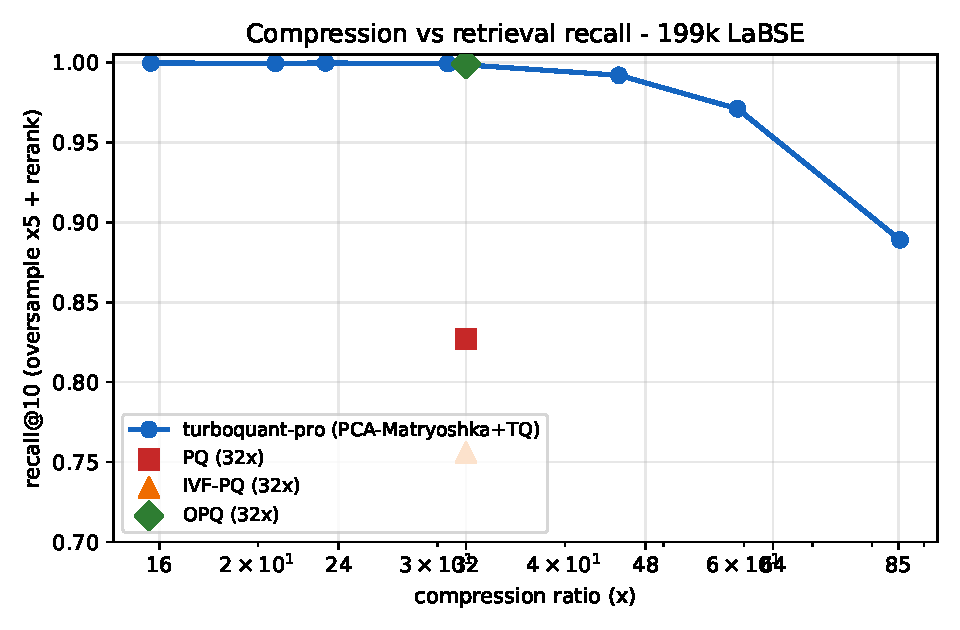
\includegraphics[width=0.95\columnwidth]{fig_pareto_tqpro.pdf}
\caption{Compression vs.\ recall@10 on 199k LaBSE (two-stage). PCA-Matryoshka
spans 16--85$\times$; PQ/IVF-PQ/OPQ are shown at 32$\times$. The frontier matches
OPQ and dominates PQ and IVF-PQ.}
\label{fig:pareto}
\end{figure}

\textbf{Ablation: rank vs.\ bits (Fig.~\ref{fig:pareto}).} At a fixed byte
budget, spending on bit-depth beats extra dimensions (PCA-128/4-bit $0.992$ $>$
PCA-256/2-bit $0.974$ at 68 bytes); the default 256-d/3-bit point
($\sim$30$\times$) is near-optimal at recall@10 $0.9993$, and even $85\times$
compression retains recall@10 $0.89$ with rerank.

\textbf{Truncatability.} On BGE-M3 (not Matryoshka-trained), na\"ive truncation
to 256-d gives cosine $0.467$ to the full vector; PCA-Matryoshka gives $0.974$ --
a $109\%$ improvement -- which is what enables the training-free pipeline to reach
OPQ-class recall.

\textbf{Scope: truncation needs a concentrated spectrum.} The truncation step helps
only when the PCA spectrum is concentrated, as it is for high-dimensional sentence
embeddings (LaBSE 768$\to$256-d retains $\sim$99\% variance). On the canonical
low-dimensional GloVe-100-angular benchmark (ann-benchmarks; 1.18M vectors, provided
ground truth), PCA-64 retains only $73\%$ of the variance and truncation \emph{hurts}:
recall@10 (+rerank) falls to $0.685$ vs PQ's $0.862$. With \emph{no} truncation at
the same byte budget, however, our scalar quantizer still wins (PCA-100+TQ2: $0.906$
vs PQ $0.862$, OPQ $0.866$). The lesson is that truncation depth should track
cumulative explained variance (e.g. $\geq 95\%$), an automatic model/data-aware choice;
PCA-Matryoshka is the right tool for high-dimensional embeddings with spectral
concentration, not for low-dimensional descriptor sets.

\textbf{Cosine is not a proxy for recall.} Across configurations, higher
cosine-to-original does not imply higher recall@10: e.g. PCA-256+TQ3 has
\emph{lower} cosine ($0.963$) yet \emph{higher} recall@10 ($78.2\%$) than
PCA-384+TQ3 ($0.979$ cosine, $76.4\%$). Compression methods should be evaluated
on task-relevant retrieval metrics, not proxy similarity.

\section{System and Reproducibility}
The method is implemented in an open-source package with connectors for
\texttt{pgvector}, FAISS, and common vector databases; the \texttt{pgvector}
path stores \emph{and searches} compressed vectors inside PostgreSQL without
decompression. A one-click notebook reproduces the compression-vs-recall
comparison on public data. % anonymized for review

\section{Conclusion}
A training-free PCA rotation makes any encoder's embeddings truncatable, and
combined with scalar quantization reaches the accuracy of the strongest learned
baseline at a fraction of the index-build cost, validated on 1M real
multilingual vectors. A batched AVX2 ADC kernel searches the compressed codes at
$7.9\times$ the speed of naive decompression with no recall loss, so the method is
simultaneously fast, compressed, and high-recall; sub-linear scaling via an IVF
coarse quantizer over the same codes is the natural next step for billion-scale
corpora.

\balance
\begin{thebibliography}{0}
\bibitem{mrl} A. Kusupati et al. Matryoshka representation learning. NeurIPS 2022.
arXiv:2205.13147.
\bibitem{turboquant} A. Zandieh, M. Daliri, M. Hadian, V. Mirrokni. TurboQuant:
Online vector quantization with near-optimal distortion rate. arXiv:2504.19874,
2025.
\bibitem{opq} T. Ge, K. He, Q. Ke, J. Sun. Optimized product quantization.
IEEE TPAMI, 2014.
\bibitem{faiss} J. Johnson, M. Douze, H. J\'egou. Billion-scale similarity search
with GPUs. IEEE Trans. Big Data, 2021.
\end{thebibliography}

\end{document}
